\section{Full Environment Results}


Among the three algorithms, only SAC delivered a working grasp policy. Therefore, we mostly evaluated the performance of the SAC algorithm's variants. We tested with different perception pipeline, different reward definition, and buffer size. Contrary to the simplified environment, we verified the algorithm's robustness on the wooden block object database. \todo{MORE}


\begin{table}[!htbp]
    \begin{tabular}{|l|l|l|l|l|}
    \hline
                                  & \multicolumn{4}{c|}{\textbf{SAC Full Environment}}                                                                                                                                                                                                                                                                                                                                  \\ \hline
                                  & \multicolumn{2}{c|}{\textbf{Floor Scene}}                                                                                                                                                & \multicolumn{2}{c|}{\textbf{Table Scene}}                                                                                                                                                \\ \hline
    \textbf{Models}               & \multicolumn{1}{c|}{\textbf{\begin{tabular}[c]{@{}c@{}}Random Objects\\ (\%)\end{tabular}}} & \multicolumn{1}{c|}{\textbf{\begin{tabular}[c]{@{}c@{}}Wooden Blocks\\ (\%)\end{tabular}}} & \multicolumn{1}{c|}{\textbf{\begin{tabular}[c]{@{}c@{}}Random Objects\\ (\%)\end{tabular}}} & \multicolumn{1}{c|}{\textbf{\begin{tabular}[c]{@{}c@{}}Wooden Blocks\\ (\%)\end{tabular}}} \\ \hline
    \textbf{SAC\_encoder\_50k}    & 65                                                                                          & 62                                                                                         & 63                                                                                          & 59                                                                                         \\ \hline
    \textbf{SAC\_encoder\_1m}     & 100                                                                                         & 95                                                                                         & 99                                                                                          & 82                                                                                         \\ \hline
    \textbf{SAC\_depth}           & 100                                                                                         & 95                                                                                         & 95                                                                                          & 23                                                                                         \\ \hline
    \textbf{SAC\_rgbd}            & 91                                                                                          & 95                                                                                         & 46                                                                                          & 17                                                                                         \\ \hline
    \textbf{SAC\_depth\_no\_curr} & 100                                                                                         & 97                                                                                         & 97                                                                                          & 64                                                                                         \\ \hline
    \textbf{SAC\_depth\_sparse}   & 99                                                                                          & 97                                                                                         & 100                                                                                         & 72                                                                                         \\ \hline
    \textbf{SAC\_depth\_no\_act}  & 95                                                                                          & 75                                                                                         & 84                                                                                          & 24                                                                                         \\ \hline
\end{tabular}
\end{table}


\begin{figure}[!htbp]
    \begin{subfigure}{0.49\textwidth}
        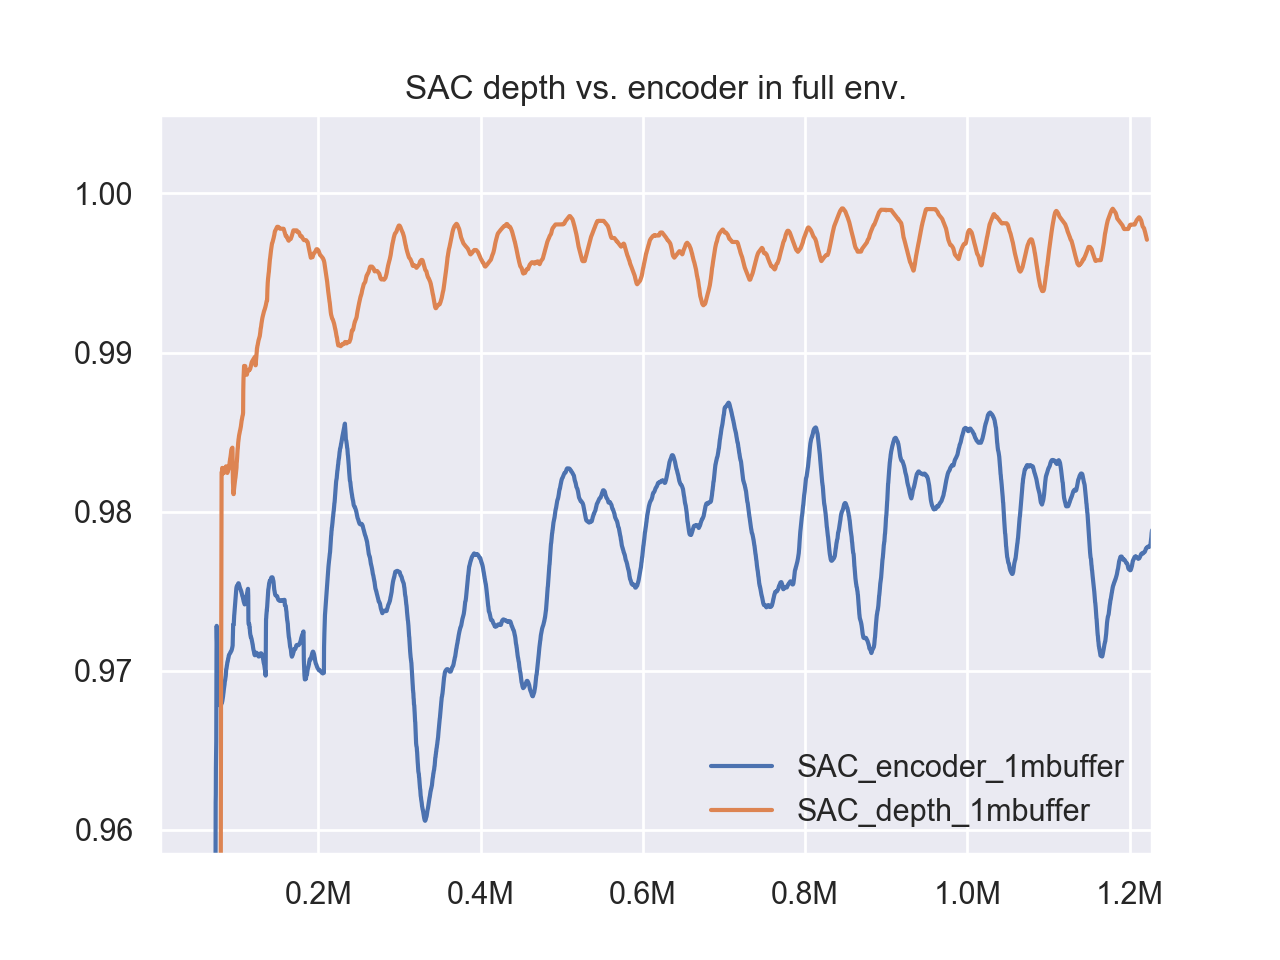
\includegraphics[width=\linewidth]{figures/SACfull/SAC_depth_vs_encoder_in_full_env}
        \caption{Table Scene} \label{fig:table}
    \end{subfigure}%
    \hspace*{\fill}   % maximize separation between the subfigures
    \begin{subfigure}{0.49\textwidth}
        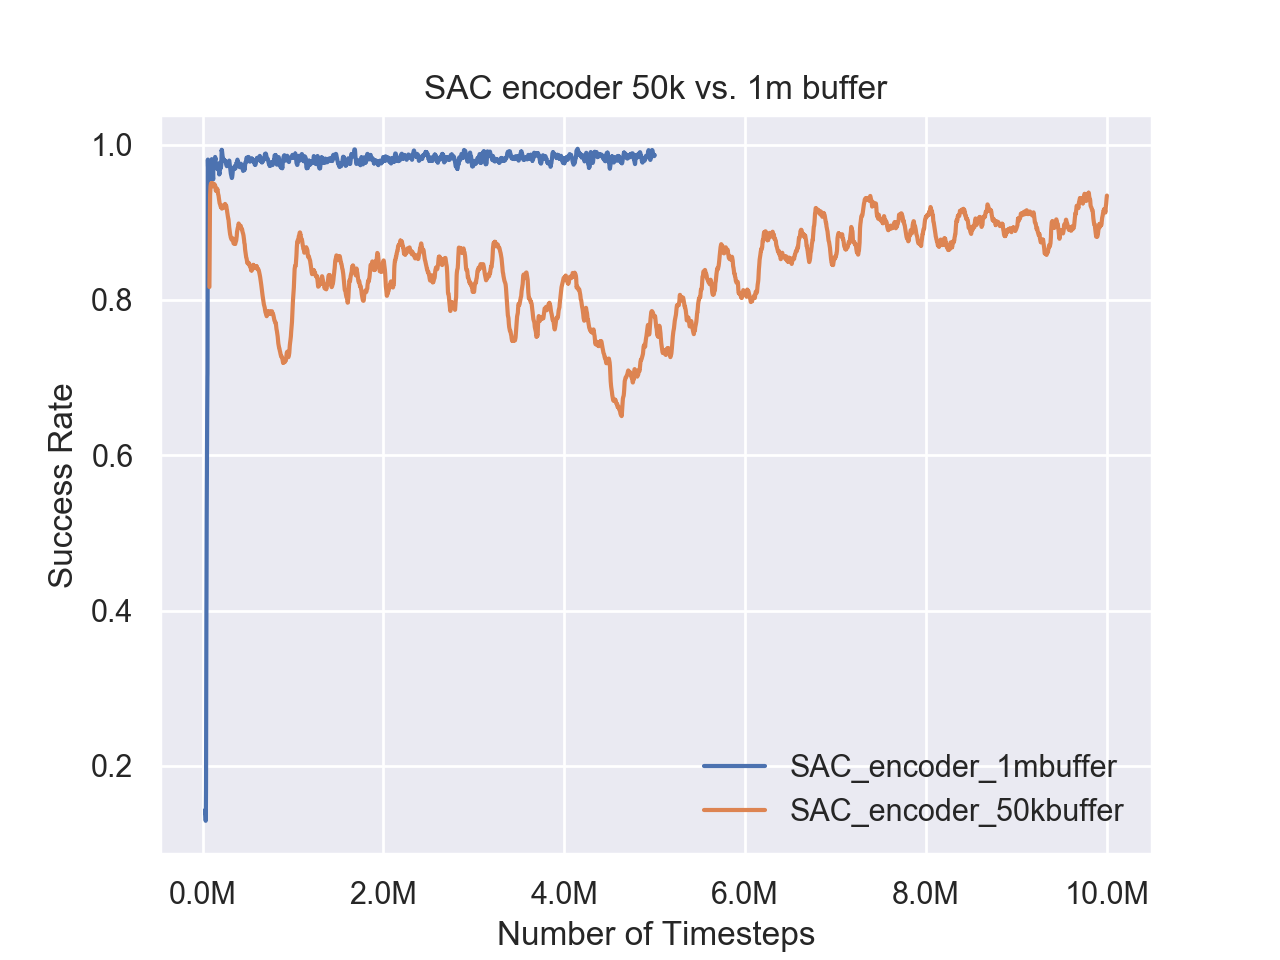
\includegraphics[width=\linewidth]{figures/SACfull/SAC_encoder_50k_vs_1m_buffer}
        \caption{Floor Scene} \label{fig:floor}
    \end{subfigure}%
    \hspace*{\fill}   % maximize separation between the subfigures


\caption{ Table and floor scenes \label{fig:scenes}}
\end{figure}

\begin{figure}[!htbp]
    \centering
        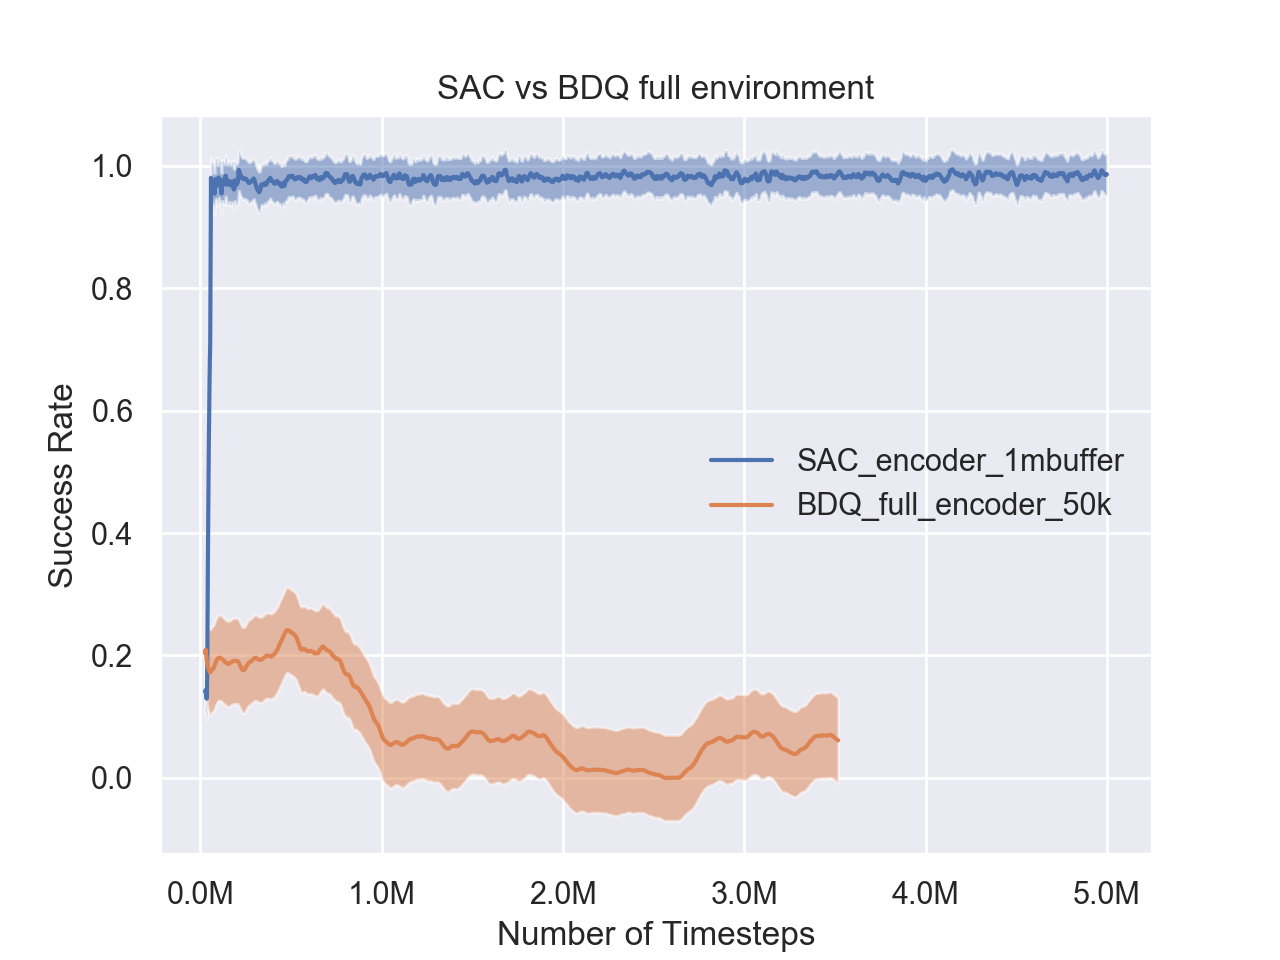
\includegraphics[width=0.4\textwidth]{figures/SACfull/SAC_vs_BDQ_full_environment}
    \caption{Different manipulation skill adopted to robotic manipulators \cite{Kroemer2019}}
    \label{fig:x manipulation_skills}
\end{figure}
